\documentclass{tufte-handout}

\title{CS294: Deep Reinforcement Learning
       \thanks{Course Instructors: Sergey Levine} \\
       \Large Lecture Notes: Policy Gradient \thanks{Author: InnerPeace}}

\date{Fall 2017\thanks{Un-official Lecture Notes}} % without \date command, current date is supplied

%\geometry{showframe} % display margins for debugging page layout

\usepackage{graphicx} % allow embedded images
  \setkeys{Gin}{width=\linewidth,totalheight=\textheight,keepaspectratio}
  \graphicspath{{notes3/fig/}} % set of paths to search for images
\usepackage{amsmath}  % extended mathematics
\usepackage{amstext}  % extended text
\usepackage{booktabs} % book-quality tables
\usepackage{units}    % non-stacked fractions and better unit spacing
\usepackage{multicol} % multiple column layout facilities
\usepackage{lipsum}   % filler text
\usepackage{fancyvrb} % extended verbatim environments
\usepackage{cancel}
\usepackage{algorithm}
\usepackage{algorithmic}
\usepackage{placeins}
\usepackage{mdframed}% http://ctan.org/pkg/mdframed
  \fvset{fontsize=\normalsize}% default font size for fancy-verbatim environments

% Standardize command font styles and environments
\newcommand{\doccmd}[1]{\texttt{\textbackslash#1}}% command name -- adds backslash automatically
\newcommand{\docopt}[1]{\ensuremath{\langle}\textrm{\textit{#1}}\ensuremath{\rangle}}% optional command argument
\newcommand{\docarg}[1]{\textrm{\textit{#1}}}% (required) command argument
\newcommand{\docenv}[1]{\textsf{#1}}% environment name
\newcommand{\docpkg}[1]{\texttt{#1}}% package name
\newcommand{\doccls}[1]{\texttt{#1}}% document class name
\newcommand{\docclsopt}[1]{\texttt{#1}}% document class option name
\newenvironment{docspec}{\begin{quote}\noindent}{\end{quote}}% command specification environment
\newcommand{\argmin}{\operatornamewithlimits{argmin}}
\newcommand{\argmax}{\operatornamewithlimits{argmax}}
\newcommand{\norm}[1]{\left\lVert#1\right\rVert}
\newcommand{\textunderscript}[1]{$_{\text{#1}}$}

\newcommand{\etal}{\textit{et al}. }
\newcommand{\ie}{\textit{i}.\textit{e}., }
\newcommand{\eg}{\textit{e}.\textit{g}. }
\newcommand{\s}{\mathbf{s}}
\newcommand{\act}{\mathbf{a}}

\allowdisplaybreaks
\setcounter{secnumdepth}{3}

\newmdtheoremenv[outerlinewidth=2,leftmargin=40,rightmargin=40,%
    backgroundcolor=lightgray,outerlinecolor=blue,innertopmargin=10pt,%
    splittopskip=\topskip,skipbelow=\baselineskip,%
    skipabove=\baselineskip,ntheorem,roundcorner=5pt]{theorem}{Snippet}[section]

\begin{document}

\maketitle% this prints the handout title, author, and date

%\printclassoptions


\textbf{Keyphrases: Policy Gradient. Variance Reduction. }\\

\noindent{}This set of notes introduces derivation of the policy gradient algorithm. We then discuss the basic variance reduction techniques like causality and baselines. Lastly, we will illustrate some examples of policy gradient which helps to understand practical considerations for policy gradients.

\section{Derivation}

Recall that the goal of RL is maximizing the expected cumulative rewards of trajectories distributed according to product of probabilities of state-action sequences:
\begin{equation}
\label{eq:1}
\underbrace{\pi_\theta(\s_1, \act_1, \cdots , \s_T, \act_T)}_{\pi_\theta (\tau)} =
  p(\s_1) \prod _{t=1}^T \big(\pi_\theta (\act_t | \s_t) p(\s_{t+1} | \s_t, \act_t)\big)
\end{equation}

\begin{equation}
\label{eq:2}
\theta^\star = \arg \max_\theta E_{\tau \sim p_\theta(\tau) }\Big[ \sum_t r(\s_t, \act_t) \Big]
\end{equation}

What we are trying to do is evaluating the expected cumulative rewards, and it's hard unless the distribution is clean like Gaussian. The straightforward solution is approximating by Monte Carlo \ie by drawing samples. For similarity, we denote the expected cumulative rewards as $J(\theta)$, and $r(\tau)$ as
the cumulative rewards over $T$ time-steps.
\[
r(\tau) = \sum_{t=1} ^ T r(\s_t, \act_t)
\]

\begin{equation}
\label{eq:3}
J(\theta) = E_{\tau \sim p_\theta(\tau) }\Big[ \sum_t r(\s_t, \act_t) \Big]
 \approx \frac{1}{N} \sum_i \sum_t r(\s_{i,t}, \act_{i,t})
\end{equation}

We generate samples from trajectory distribution $p_\theta(\tau)$, and approximating $J(\theta)$ by averaging. The more samples, the more accurate it
will be. Or we can also rewrite $J(\theta)$ as the integral of probability of trajectory times the reward according to the definition of expectation.
\begin{equation}
\label{eq:4}
J(\theta) = \int \pi_\theta (\tau) r(\tau) d\tau
\end{equation}

Following the intuition of DL, firstly, we evaluate the gradients of the objective w.r.t the parameters, then, applying gradient descent or ascent to
improve the objective value. Before derivation, we introduce a convenient identity, for any distribution $p_\theta (\tau)$:
\begin{equation}
\label{eq:5}
p_\theta(\tau) \nabla_\theta \log p_\theta(\tau) = p_\theta(\tau) \frac{\nabla _ \theta p_\theta (\tau)}{p_\theta (\tau)}
= \nabla _ \theta p_\theta (\tau)
\end{equation}
Just using the property of derivation of log function.
The gradient of $J(\theta)$ w.r.t parameters of policy networks is:

\begin{align}
\label{eq:6}
\nabla _\theta J(\theta) &= \int \nabla _\theta \pi_\theta (\tau) r(\tau) d(\tau) \notag \\
&= \int \pi_\theta (\tau) \frac{\nabla _ \theta \pi_\theta (\tau)}{\pi_\theta (\tau)} r(\tau) d(\tau)\notag \\
& = \int \pi_\theta (\tau)\nabla _ \theta \log(\pi_\theta (\tau)) r(\tau) d(\tau)\notag \\
& = E_{\tau \sim p_\theta(\tau) } \big[\nabla _ \theta \log(\pi_\theta (\tau)) r(\tau)\big  ]
\end{align}
We take the gradients into the integral with the property that differentiation is linear, and replace $\nabla _\theta \pi_\theta (\tau)$
 with the identity of equation \ref{eq:5}, then rewrite it with form of expectation. To get the derivation of log of probability of trajectory,
 we can take \emph{logarithm} to both sides of equation \ref{eq:1}:

\begin{align}
\label{eq:7}
\log \pi_\theta(\tau) &= \log p(\s_1) + \sum_{t=1}^T \log \pi_\theta(\act_t| \s_t) + \log p(\s_{t+1} | \s_t, \act_t) \notag \\
\nabla_\theta \log \pi_\theta(\tau) &= \cancel{\log p(\s_1)} + \sum_{t=1}^T \nabla_\theta \log \pi_\theta(\act_t| \s_t) +
\cancel{\log p(\s_{t+1} | \s_t, \act_t)} \notag \\
 & = \sum_{t=1}^T \nabla_\theta \log \pi_\theta(\act_t| \s_t)
\end{align}

Then we substitute $\nabla_\theta \log \pi_\theta(\tau)$ of equation \ref{eq:6} with result of equation \ref{eq:7}:

\begin{align}
\label{eq:8}
\nabla _\theta J(\theta) & = E_{\tau \sim p_\theta(\tau) } \Big[ \Big(\sum_{t=1}^T \nabla_\theta \log \pi_\theta(\act_t| \s_t) \Big)
  \Big( \sum_{t=1}^T r(\s_t, \act_t) \Big)\Big] \notag \\
  & \approx \frac{1}{N} \sum_{i=1} ^ {N} \bigg[\Big(\sum_{t=1}^T \nabla_\theta \log \pi_\theta(\act_{i,t} | \s_{i,t}) \Big)
  \Big( \sum_{t=1}^T r(\s_{i,t}, \act_{i,t}) \Big) \bigg]
\end{align}
The wonderful thing happens to equation \ref{eq:8} is that the gradients of the objective does not depend on the probability of initial state and
 transition distribution. If we can sample from the dynamical system, then we can evaluate the gradient w.r.t to policy $\pi$ and improve policy with
 gradient updating:

 \begin{equation}
 \label{eq:9}
 \theta \quad \leftarrow \quad \theta + \alpha \nabla _\theta J(\theta)
 \end{equation}

Combining these components together to the \emph{REINFORCE algorithm}:

\begin{algorithm}
  \caption{REINFORCE algorithm}
  \label{algo:reinforce}
  \begin{algorithmic}[1]
  \STATE sample $\{\tau ^ i \} $ from $\pi_\theta(\act_t | \s_t)$ by running the policy. \\
  \STATE $\nabla _\theta J(\theta) \approx 1/N \sum_{i=1} ^ {N} \bigg[\Big(\sum_{t=1}^T \nabla_\theta \log \pi_\theta(\act_t| \s_t) \Big)
  \Big( \sum_{t=1}^T r(\s_t, \act_t) \Big) \bigg]$ \\
  \STATE $ \theta \leftarrow \theta + \alpha \nabla _\theta J(\theta)$ \\
  \STATE Back to step 1: policy sampling.
  \end{algorithmic}
\end{algorithm}

For \emph{POMDP}, since we don't use Markov Property during derivation, we can apply policy gradient to \emph{POMDP} by substituting $\s_{i,t}$
with $\mathbf{o}_{i,t}$ and without further modification.

To dive deeper, if we apply maximum likelihood as the objective in imitation learning, then the gradient should be:

\begin{equation}
\label{eq:10}
\nabla_\theta J_{ML} (\theta) \approx \frac{1}{N} \sum_{i=1} ^ {N} \Big(\sum_{t=1}^T \nabla_\theta \log \pi_\theta(\act_t| \s_t) \Big)
\end{equation}
Compare it with equation \ref{eq:8}, they are extremely similar to each other except that policy gradient in equation \ref{eq:8} is weighted by the cumulative sum of rewards of the trajectory, and the sum of rewards could be positive or negative. In general, \emph{Maximum Likelihood} will always increase the probability of trajectory in all the data, while policy gradient prefer the trajectory with high reward and increase the probabilities of the
these trajectories, decrease the probability of trajectories with low reward.

\subsection{Example: Gaussian Policies}
For the \emph{Humanoid} task in gym of openai where the robot has continuous actions, we need the output of policy to be distribution over continuous vector. We choose to use conditional Gaussian and neural network to look at the state $\s_t$ and output the mean of distribution, and for the covariance matrix, we can either use constant like 1 and only care about the mean, or take it as a trainable variable in practice.
\begin{equation}
  \label{eq:11}
  \pi_\theta(\act_t | \s_t) = \mathcal{N} (f_{NN} (\s_t); \Sigma)
\end{equation}
Where we use the multivariate Gaussian distribution \thanks{Refer \href{https://people.eecs.berkeley.edu/~jordan/courses/260-spring10/other-readings/chapter13.pdf}{\underline{lecture notes of Multivariate Gaussian}} by Jordan, UCB for more details} which is commonly expressed in terms of parameters $\mu$ and $\Sigma$, where $\mu$ is an $n \times 1$
vector and $\Sigma$ is an $n \times n$, symmetric matrix.
\begin{equation}
  \label{eq:12}
  p(x | \mu, \Sigma) = \frac{1}{ (2\pi)^{n/2} |\Sigma| ^{1/2}} \exp \bigg\{ - \frac{1}{2}(x- \mu)^T \Sigma ^{-1} (x- \mu) \bigg\}
\end{equation}
Suppose that we have an i.i.d distributed data set $\mathcal{D} = \{x_1, x_2, \cdots, x_N \}$, and we form the log likelihood function by taking the logarithm of product of N Gaussians:
\begin{align}
\label{eq:12}
\log(\mu, \Sigma | \mathcal{D})
& = \log \big(p(x_1 | \mu, \Sigma)p(x_2 | \mu, \Sigma) \cdots p(x_N | \mu, \Sigma) \big) \notag \\
& = - \frac{N}{2} \log | \Sigma | - \frac{1}{2} \sum_{i=1} ^N (x_i - \mu)^T \Sigma ^{-1} (x_i - \mu) + \text{const}
\end{align}

\indent If we take $\Sigma$ as constant and  substitute with policy at time-step $t$:
\begin{equation}
\label{eq:13}
\log \pi_\theta (\act_t | \s_t) = -\frac{1}{2} (\act_t - f(\s_t))^T \Sigma ^{-1} (\act_t - f(\s_t)) + \text{const}
\end{equation}
\indent Along with the properties:
\begin{align}
(AB)^T &= B^T \cdot A^T \\
\frac{\partial \mathbf{u}^T \mathbf{v}}{\partial \mathbf{v}} &=\frac{\partial \mathbf{v}^T \mathbf{u}}{\partial \mathbf{v}} = \mathbf{u}
\end{align}

\indent Then differentiate equation \ref{eq:13} w.r.t parameters $\theta$
\begin{equation}
\label{eq:17}
\nabla_\theta \log \pi_\theta(\act_t| \s_t) = \big(\act_t - f(\s_t) \big) ^T \Sigma ^{-1} \frac{df}{d\theta}
\end{equation}
\indent Substitute $\nabla_\theta \log \pi_\theta(\act_t| \s_t)$ in equation \ref{eq:8}, we obtain the the gradient w.r.t parameters of policy and improve policy by gradient updating.

\section{Problems of Policy Gradient}
In general, there are two problems in policy gradient.


\begin{figure*}
\caption{Toy example of High Variance problem}
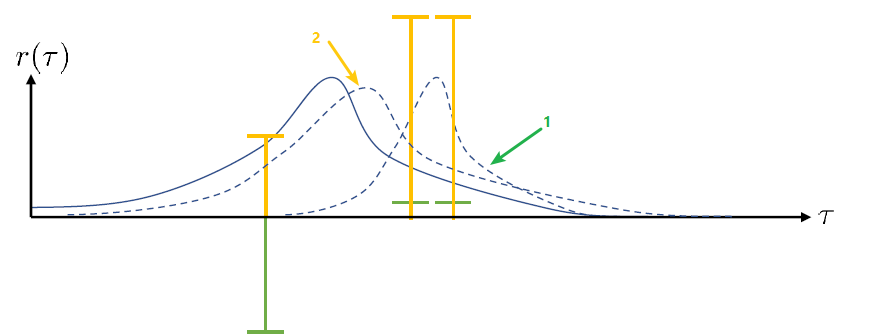
\includegraphics[width=14cm]{variance}
\label{fig:variance}

\end{figure*}

Figure \ref{fig:variance} illustrates a simplified example where the trajectory is 1-D along x-axis, and the y-axis indicates the rewards of specific trajectory, the funny blue curve is the policy \ie the distribution of trajectories. Firstly, we sample 3 trajectories and represent their rewards with green bar where one sample has big negative reward and the other two have small positive rewards. Policy gradient algorithm will try to shift to the right (indicated by number 1) so that the distribution has more mass on the good trajectories. Then if we add a constant to the reward function, the results of sampled trajectories look like the yellow bar. Besides, adding constant to reward has no impact on gradient, we will prove it later. The situation is that the policy gradient will increase the probabilities of all the three samples, and the curve will move slightly to the right, even choose to increase its variance to become wider
(curve indicated by number 2). This example shows that two kinds of rewards which are functionally equivalent but produce different updates. The process will highly depend on the initial position of the distribution if we push down the two positive rewards to zero. This is referred as the \emph{High Variance}. One straightforward way to address this is to take infinite samples where all the differences will eventually cancel out.

Another problem is \emph{slow convergence}. Suppose another one-dimensional policy which distributed according to Gaussian distribution:
\[
\pi_\theta (a_t | s_t) = \frac{1}{\sqrt{2\pi} \sigma} \exp \bigg\{ - \frac{(a_t - ks_t) ^ 2}{2 \sigma^2} \bigg\}
\]
The logarithm of policy is:
\[\log  \pi_\theta (a_t | s_t) =- \frac{1}{2 \sigma^2}(a_t - ks_t) ^ 2  + \text{const} \]
And we set the reward as:
\[
r(s_t, a_t) = -s_t^2 - a_t ^2
\]
\indent Where the gradient tries to decrease the state and take small action. And the parameters of policy are linear constant $k$ and variance $\sigma$,
$\theta = (k, \sigma)$. Figure \ref{fig:slow-converge} indicates that the gradient always want to decrease $\sigma$, since decreasing the variance will
help to keep from choosing big action. At the same time, the objective also want to decrease $k$ to lower the mean of the distribution. But the problem is that the gradient w.r.t $\sigma$ is much larger than that of $k$, and as $\sigma$ decreasing, gradient becomes larger and $\sigma$ decrease even faster. In contrast, the gradient w.r.t $k$ becomes smaller which results in \emph{slow convergence}. Later, we will introduce \emph{natural gradient estimation} to address the problem.
\begin{marginfigure}
  \centering
  \caption{Illustration of gradients w.r.t $\theta =(k, \sigma)$, image from Peters \& Schaal 2008.}
  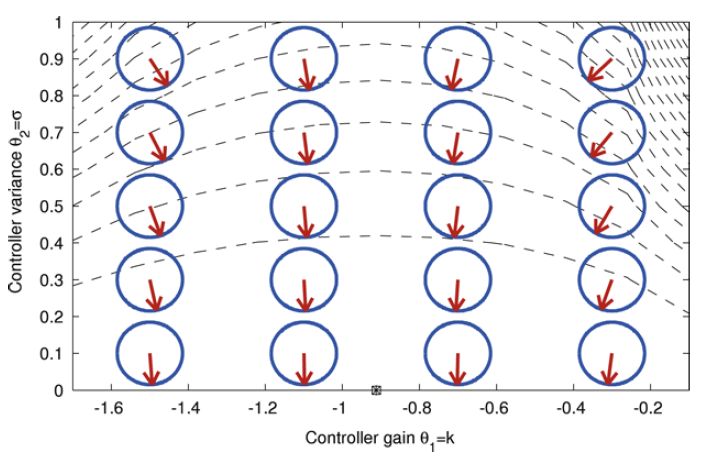
\includegraphics[width=\linewidth]{slow}
  \label{fig:slow-converge}
\end{marginfigure}

\subsection{Causality}
For the problem of \emph{High Variance}, there are two methods to address it.

The first idea is \emph{causality} which means policy at time $t'$ cannot affect reward at time $t$ when $t < t'$. It's intuitive \eg what I do today won't change what happened yesterday as time flows forward. With this idea, we obtain a better policy gradient estimator by rewriting equation \ref{eq:8} as:
\begin{equation}
\label{eq:18}
\nabla _\theta J(\theta) \approx \frac{1}{N} \sum_{i=1} ^ {N} \bigg[\sum_{t=1}^T \nabla_\theta \log \pi_\theta(\act_{i,t}| \s_{i,t})
  \Big( \sum_{t'=t}^T r(\s_{i, t'}, \act_{i, t'}) \Big) \bigg]
\end{equation}

Where we distribute the sum of rewards into the sum of gradients and compute the cumulative rewards starting from time-step $t$, which is referred as \emph{reward to go}. The intuition is that the variance goes down with summing over fewer numbers. We can denote \emph{reward to go} w.r.t Q-function:
\begin{equation}
\label{eq:19}
Q_{i,t} = \sum_{t' = t} ^T r(\s_{i, t'}, \act_{i, t'})
\end{equation}
And this is trivial to compute if you starting from the end of the sequences, people always use this idea in practice.

\subsection{Baselines}
The "vanilla" policy gradient change the probabilities of trajectories based how good or bad there are w.r.t the reward, and the toy example shows that adding constant to reward could be problematic. Is there another metric to "good" or "bad" of the trajectory which are more stable? The idea is changing the probability based on how better or worse the trajectory is than the average \thanks{Refer to \href{https://www.sciencedirect.com/science/article/pii/S0893608008000701}{\underline{Peters \& Schaal 2008}} for overview of optimal baselines and natural gradient}. For simplicity, we rewrite equation \ref{eq:8} w.r.t trajectory $\tau$.
\begin{align*}
\label{eq:20}
\nabla _\theta J(\theta)
 & \approx \frac{1}{N} \sum_{i=1} ^ {N} \bigg[\Big(\sum_{t=1}^T \nabla_\theta \log \pi_\theta(\act_{i,t} | \s_{i,t}) \Big)
  \Big( \sum_{t=1}^T r(\s_{i,t}, \act_{i,t}) \Big) \bigg] \notag \\
 & = \frac{1}{N} \sum_{i=1} ^ {N}\nabla_\theta \log \pi_\theta(\tau) r(\tau)
\end{align*}
Then we substract reward of each trajectory with baseline $b$:
\[
b = \frac{1}{N} \sum_{i=1} ^ N r(\tau)
\]
\begin{equation}
\label{eq:21}
 \nabla _\theta J(\theta) \approx \frac{1}{N} \sum_{i=1} ^ {N}\nabla_\theta \log \pi_\theta(\tau) [r(\tau) - b]
\end{equation}
Does adding the baseline mathematically legitimate? The result is that adding a constant to the reward, the expectation of gradient is unbiased.
The derivation as follows:
\begin{equation}
\label{eq:22}
E[\nabla_\theta \log \pi_\theta(\tau) b ] = \int \pi_\theta(\tau) \nabla_\theta \log \pi_\theta(\tau) b d\tau
 = \int \nabla_\theta \pi_\theta (\tau) b d \tau = b \nabla _\theta \int \pi_\theta (\tau) d \tau =  b \nabla_\theta 1 = 0
\end{equation}
Where we applied the identity in equation \ref{eq:5}, and took grad operation and constant $b$ outside the integral, finally, the integral of probability over trajectories is 1. In fact, the average baseline is not the best baseline, but it's pretty good. What's the optimal baseline? what we are trying to do is reducing the variance, and mathematically, variance of variable $x$ is:
\[
\text{Var}[x] = E[x^2] - E[x] ^2
\]
For policy gradient we substitute $x$ with $\nabla_\theta \log \pi_\theta(\tau) (r(\tau) - b)$ and the expectation is:
\begin{equation}
\label{eq:23}
\nabla _\theta J(\theta) = E_{\tau \sim \pi_\theta (\tau)} [\nabla_\theta \log \pi_\theta(\tau) (r(\tau) - b)]
\end{equation}
The variance is
\begin{equation}
\label{eq:24}
\text{Var} =
E_{\tau \sim \pi_\theta (\tau)} [(\nabla_\theta \log \pi_\theta(\tau) (r(\tau) - b)) ^ 2] -
E_{\tau \sim \pi_\theta (\tau)} [\nabla_\theta \log \pi_\theta(\tau) (r(\tau) - b)] ^ 2
\end{equation}
We proved that adding constant to reward has no impact on gradient with equation \ref{eq:22}, which means:
\begin{equation}
\label{eq:25}
E_{\tau \sim \pi_\theta (\tau)} [\nabla_\theta \log \pi_\theta(\tau) (r(\tau) - b)] ^ 2 =
E_{\tau \sim \pi_\theta (\tau)} [\nabla_\theta \log \pi_\theta(\tau) r(\tau) ] ^ 2
\end{equation}
We substitute grad log $pi$ with $g(\tau)$:
\[
g(\tau) = \nabla_\theta \log \pi_\theta(\tau)
\]
Then we differentiate Var w.r.t to baseline $b$, ans set it to 0:
\begin{align}
\label{eq:26}
\frac{d \text{Var}}{db} & = \frac{d}{db} E[g(\tau) ^ 2 (r(\tau) - b) ^2] \notag \\
& = \frac{d}{db} (\cancel{E[g(\tau)^2 r(\tau)^2]} - 2E[g(\tau)^2 r(\tau) b] + b^2 E[g(\tau) ^ 2]) \notag \\
& = -2 E[g(\tau) ^ 2 r(\tau)] + 2b E[g(\tau) ^ 2] \notag \\
& = 0
\end{align}
The optimal baselines is:
\begin{equation}
\label{eq:27}
b = \frac{E[g(\tau) ^2 r(\tau)]}{E[g(\tau) ^ 2]}
\end{equation}
This is just expected reward, but weighted by gradient magnitudes. And in practice, average reward works just fine.

\section{Importance Sampling}
We introduced the concept of \emph{on-policy} in notes of lecture 3. And policy gradient is one of the instances where we have to sample new trajectories each time we update the policy network. The problem is that neural networks change only a little bit with each gradient update, results in sampling inefficient. So can we take advantage of the old samples? The idea is we can sample from other distribution instead of the new policy $\pi_\theta(\tau)$ with \emph{importance sampling}.

Suppose that we want to estimate expectation of $f(x)$ with $x$ distributed according to $p(x)$, but if we have $x$ from distribution $q(x)$, we still calculate the expectation with \emph{importance sampling}:
\begin{align}
\label{eq:28}
E_{x \sim p(x)} [f(x)] & = \int p(x) f(x) dx \notag \\
& = \int \frac{q(x)}{q(x)} p(x) f(x) dx \notag \\
& = \int q(x) \frac{p(x)}{q(x)} f(x) dx \notag \\
& = E_{x \sim q(x)} \bigg[\frac{p(x)}{q(x)} f(x)\bigg]
\end{align}
Where we sample $x$ from distribution $q(x)$ and insert the correction $\frac{p(x)}{q(x)}$ which is also referred as \emph{importance wight}. We can apply this idea to policy sampling where we sample from $\pi'(\tau)$ instead of $\pi(\tau)$:
\begin{equation}
\label{eq:29}
J(\theta) = E_{\tau \sim \pi'(\tau)} \bigg[\frac{\pi_\theta(\tau)}{\pi'(\tau)} r(\tau) \bigg]
\end{equation}
And recall that probability of trajectory is the product of probabilities of state-action sequences, then the \emph{importance weight} in equation \ref{eq:29} is:
\begin{align}
\label{eq:30}
\frac{\pi_\theta (\tau))}{\pi'(\tau)} &  =  \frac{\cancel{p(\s_1)}\prod _{t=1}^T \big(\pi_\theta (\act_t | \s_t) \cancel{p(\s_{t+1} | \s_t, \act_t)}\big)}
{\cancel{p(\s_1)}\prod _{t=1}^T \big(\pi' (\act_t | \s_t) \cancel{p(\s_{t+1} | \s_t, \act_t)}\big)} \notag \\
& =  \frac{\prod _{t=1}^T \pi_\theta (\act_t | \s_t)}{\prod _{t=1}^T \pi' (\act_t | \s_t)}
\end{align}
In theory, with sampling from $\pi'(\tau)$, we can evaluate new policy $\pi_\theta(\tau)$ without samples. Besides, we derive policy gradient with importance sampling. Firstly, we rewrite equation \ref{eq:29} with policy $\pi_\theta (\tau)$ and $\pi_{\theta'} (\tau) $:
\begin{equation}
\label{eq:31}
J(\theta') = E_{\tau \sim \pi_\theta(\tau)} \bigg[\frac{\pi_{\theta'}(\tau)}{\pi_\theta(\tau)} r(\tau) \bigg]
\end{equation}
And we estimate gradient w.r.t new parameter $\theta'$:
\begin{align}
\label{eq:32}
\nabla _ {\theta'} J(\theta') & = E _{\tau \sim \pi_{\theta}(\tau)} \bigg[\frac{\nabla _{\theta'} \pi_{\theta'}(\tau)}{\pi_\theta(\tau)} r(\tau) \bigg] \notag \\
& = E _{\tau \sim \pi_{\theta}(\tau)} \bigg[\frac{\pi_{\theta'} (\tau)}{\pi_\theta(\tau)}\nabla _{\theta'} \log \pi_{\theta'}(\tau) r(\tau) \bigg]
\end{align}
Where we applied the identity in equation \ref{eq:5}. And we estimate the gradient locally at $\theta = \theta'$:
\begin{equation}
\label{eq:33}
\nabla _ {\theta} J(\theta)
= E_{\tau \sim \pi_{\theta}(\tau)} \bigg[\cancel{\frac{\pi_{\theta} (\tau)}{\pi_{\theta}(\tau)}}
\nabla _{\theta} \log \pi_{\theta}(\tau) r(\tau) \bigg]
\end{equation}
This is just what we derived earlier. What if $\theta \neq \theta'$? We can plug the result of equation \ref{eq:30} into equation \ref{eq:32}:
\begin{equation}
\label{eq:34}
\nabla _ {\theta'} J(\theta')
= E _{\tau \sim \pi_{\theta}(\tau)} \bigg[
\bigg( \frac{\prod _{t=1}^T \pi_{\theta'} (\act_t | \s_t)}{\prod _{t=1}^T \pi_\theta (\act_t | \s_t)}\bigg)
\bigg( \sum_{t=1}^T \nabla_{\theta'} \log \pi_{\theta'}(\act_{i,t}| \s_{i,t}) \bigg)
  \Big( \sum_{t'=1}^T r(\s_{i, t'}, \act_{i, t'}) \Big) \bigg]
\end{equation}
And we can also apply the idea of \emph{causality}: only the importance weight up to current time-step is helpful as future actions don't affect current weight and replace $r(\tau)$ with reward to go.
\begin{equation}
\label{eq:35}
\nabla _ {\theta'} J(\theta')
= E _{\tau \sim \pi_{\theta}(\tau)} \bigg[
\bigg( \sum_{t=1}^T \nabla_{\theta'} \log \pi_{\theta'}(\act_{i,t}| \s_{i,t}) \bigg)
\bigg( \frac{\prod _{t'=1}^t \pi_{\theta'} (\act_{t'} | \s_{t'})}{\prod _{t'=1}^t \pi_\theta (\act_{t'} | \s_{t'})}\bigg)
  \Big( \sum_{t'=t}^T r(\s_{i, t'}, \act_{i, t'}) \Big) \bigg]
\end{equation}
However the product of importance weight is exponential in time-steps which leads to zero or infinite when time-step $t$ is large. We will dive deeper in following lecture to address the problem, intuitively, we can rewrite the objective with converting MDP into \emph{Markov Chain} as discussed in lecture 2:
\begin{align}
\label{eq:36}
J(\theta) & = \sum_{t=1} ^ T E_{(\s_t, \act_t)\sim p_\theta (\s_t, \act_t)} \big[r(\s_t, \act_t) \big] \notag \\
& = \sum_{t=1} ^ T E_{\s_t \sim p_\theta (\s_t)} \big[ E_{\act_t \sim \pi_\theta (\s_t, \act_t)}[r(\s_t, \act_t) ] \big]
\end{align}
Where we divide it into expectation over two distributions: one over probability of states and another one over policy. And for the new parameter $\theta'$,
we can sample from distributions based on parameter $\theta$ and apply importance sampling to equation \ref{eq:36}:
\begin{equation}
\label{eq:37}
J(\theta')
 = \sum_{t=1} ^ T E_{\s_t \sim p_\theta (\s_t)} \bigg[ \frac{p_{\theta'} (\s_t)}{p_\theta(\s_t)}
 E_{\act_t \sim \pi_\theta (\s_t, \act_t)}\bigg[\frac{\pi_{\theta'} (\s_t, \act_t)}{\pi_\theta (\s_t, \act_t)} r(\s_t, \act_t) \bigg] \bigg]
\end{equation}
The new objective without the product of importance weight seems practical, but it's more complicated which requiring the probability of a particular state. Later, we will learn how cross out the importance wight over probability of state reasonably.

In practice, we should keep in mind that policy gradient has high variance which is noisy and larger batches helps to reduce the variance. Adaptive step size rule like Adam work fine, but we will learn more policy gradient-specific learning rate adjustment methods later.

\section{Suggested Readings}
\begin{itemize}
  \item [\textbf{Classic Papers}]
  \item Williams (1992). Simple statistical gradient-following algorithms for connectionist reinforcement learning: introduce REINFORCE algorithm:
  introduces REINFORCE algorithm. \href{http://www-anw.cs.umass.edu/~barto/courses/cs687/williams92simple.pdf}{\underline{link}}.
  \item Baxter \& Bartlett (2001). Infinite-horizon policy-gradient estimation: temporally decomposed policy gradient.
  \href{https://www.jair.org/media/806/live-806-1942-jair.pdf}{\underline{link}}.
  \item Peters \& Schaal (2008). Reinforcement learning of motor skills with policy gradients: overview of optimal baselines and natural gradient.
  \href{http://www.kyb.mpg.de/fileadmin/user_upload/files/publications/attachments/Neural-Netw-2008-21-682_4867%5b0%5d.pdf}{\underline{link}}.
  \item [\textbf{Deep Reinforcement Learning}]
  \item Levine \& Koltun (2013). Guided policy search: deep RL with importance sampled policy gradient.
  \href{https://graphics.stanford.edu/projects/gpspaper/gps_full.pdf}{\underline{link}}.
  \item Schulman et al. (2015). Trust region policy optimization: deep RL with natural gradient and adaptive step size.
  \href{https://arxiv.org/abs/1502.05477}{\underline{link}}.
  \item Schulman et al. (2017).  Proximal policy optimization algorithms: deep RL with importance sampled policy gradient.
  \href{https://arxiv.org/abs/1707.06347}{\underline{link}}.

\end{itemize}



% \begin{theorem}
% \begin{verbatim}

% # Update rule for Adam
% m = beta1*m + (1-beta1)*dx
% v = beta2*v + (1-beta2)*(dx**2)
% x += - learning_rate * m / (np.sqrt(v) + eps)
% \end{verbatim}
% \label{snip:adam}
% \end{theorem}


\end{document}
